% this is a simplified version of 
% https://github.com/yihui/knitr/blob/master/inst/examples/knitr-beamer.Rnw
\documentclass{beamer}\usepackage[]{graphicx}\usepackage[]{color}
%% maxwidth is the original width if it is less than linewidth
%% otherwise use linewidth (to make sure the graphics do not exceed the margin)
\makeatletter
\def\maxwidth{ %
  \ifdim\Gin@nat@width>\linewidth
    \linewidth
  \else
    \Gin@nat@width
  \fi
}
\makeatother

\definecolor{fgcolor}{rgb}{0.345, 0.345, 0.345}
\newcommand{\hlnum}[1]{\textcolor[rgb]{0.686,0.059,0.569}{#1}}%
\newcommand{\hlstr}[1]{\textcolor[rgb]{0.192,0.494,0.8}{#1}}%
\newcommand{\hlcom}[1]{\textcolor[rgb]{0.678,0.584,0.686}{\textit{#1}}}%
\newcommand{\hlopt}[1]{\textcolor[rgb]{0,0,0}{#1}}%
\newcommand{\hlstd}[1]{\textcolor[rgb]{0.345,0.345,0.345}{#1}}%
\newcommand{\hlkwa}[1]{\textcolor[rgb]{0.161,0.373,0.58}{\textbf{#1}}}%
\newcommand{\hlkwb}[1]{\textcolor[rgb]{0.69,0.353,0.396}{#1}}%
\newcommand{\hlkwc}[1]{\textcolor[rgb]{0.333,0.667,0.333}{#1}}%
\newcommand{\hlkwd}[1]{\textcolor[rgb]{0.737,0.353,0.396}{\textbf{#1}}}%
\let\hlipl\hlkwb

\usepackage{framed}
\makeatletter
\newenvironment{kframe}{%
 \def\at@end@of@kframe{}%
 \ifinner\ifhmode%
  \def\at@end@of@kframe{\end{minipage}}%
  \begin{minipage}{\columnwidth}%
 \fi\fi%
 \def\FrameCommand##1{\hskip\@totalleftmargin \hskip-\fboxsep
 \colorbox{shadecolor}{##1}\hskip-\fboxsep
     % There is no \\@totalrightmargin, so:
     \hskip-\linewidth \hskip-\@totalleftmargin \hskip\columnwidth}%
 \MakeFramed {\advance\hsize-\width
   \@totalleftmargin\z@ \linewidth\hsize
   \@setminipage}}%
 {\par\unskip\endMakeFramed%
 \at@end@of@kframe}
\makeatother

\definecolor{shadecolor}{rgb}{.97, .97, .97}
\definecolor{messagecolor}{rgb}{0, 0, 0}
\definecolor{warningcolor}{rgb}{1, 0, 1}
\definecolor{errorcolor}{rgb}{1, 0, 0}
\newenvironment{knitrout}{}{} % an empty environment to be redefined in TeX

\usepackage{alltt}
\IfFileExists{upquote.sty}{\usepackage{upquote}}{}
\begin{document}

\title{Introducci\'on a la Gen\'omica \\ UNAL nov 2017}
\author{Alejandro C\'aceres \\ ISGlobal, Barcelona}


\maketitle
% very important to use option [fragile] for frames containing code output!

\begin{frame}[fragile]
\frametitle{Genome-wide association studies}

En los estudios de asociaci\'on gen\'etica se prueba la correlaci\'on (associaci\'on) entre los SNPs y un fenotipo de inter\'es. Siven para

\begin{itemize}
\item identificar variantes gen\'eticos que den pistas sobre el desarrollo del fenotipo (enfermedad)
\item medir la carga gen\'etica (heredabilidad) de un fenotipo
\item crear modelos de riezgo gen\'etico que predigan la probabilidad de desarrollar una enfermedad. 
\item para ver los variantes funcionales que afectan  endofenotipos como expresi\'on genica (eQTls) 
\end{itemize}

\end{frame}


\begin{frame}[fragile]
\frametitle{Genome-wide association studies}
Una Gran cantidad de GWAS se han hecho hasta el momento. Se puden consultar en GWAS catalog
\begin{figure}[htbp]
\begin{center}
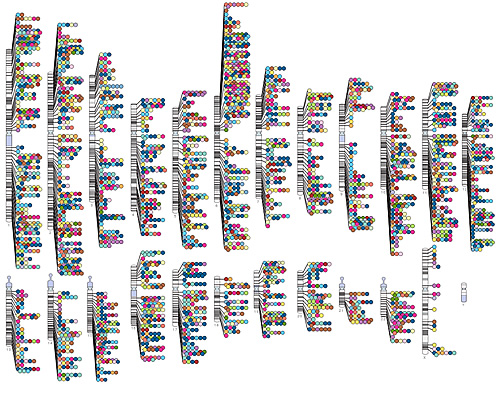
\includegraphics[width=.5\linewidth]{gwasw.jpg}
\end{center}
\end{figure}
\end{frame}




\begin{frame}[fragile]
\frametitle{Genome-wide association studies}
Una Gran cantidad de GWAS se han hecho hasta el momento. Se puden consultar en GWAS catalog
\begin{figure}
\begin{center}

\includegraphics[width=.5\linewidth]{cat.png}
\end{center}
\end{figure}
\end{frame}

\begin{frame}[fragile]
\frametitle{Genome-wide association studies}
Ejercicio: 
\begin{itemize}
\item buscar en el GWAS catalog los resultados de estudios de Alzheimer's.
\item buscar cuales GWAS han encontrado variantes geneticos en BRCA1
\end{itemize}

\end{frame}


\begin{frame}[fragile]
\frametitle{Software}

Han una gran cantidad de software para hacer estos an\'alisis
\begin{itemize}
\item PLINK, rapido pero por linea de comandos. Da poca flexibilidad 
\item snpStats mas lento pero se pueden aprovechar los paquetes de R
\item codigo en R. Se puede usar cualquier tipo de test. Lo ideal es paralelizar.
\item snpAssoc. Tambien en R. Para estudios con n\'umero limitado de SNPs pero prueba todos lo modelos geneticos y ajusta por el n\'umero de tests.
\end{itemize}
\end{frame}

\begin{frame}[fragile]
\frametitle{PLINK}
PLINK tiene unos datos de prueba y y unos ejemplos de analisis sobre ellos

\begin{figure}
\begin{center}
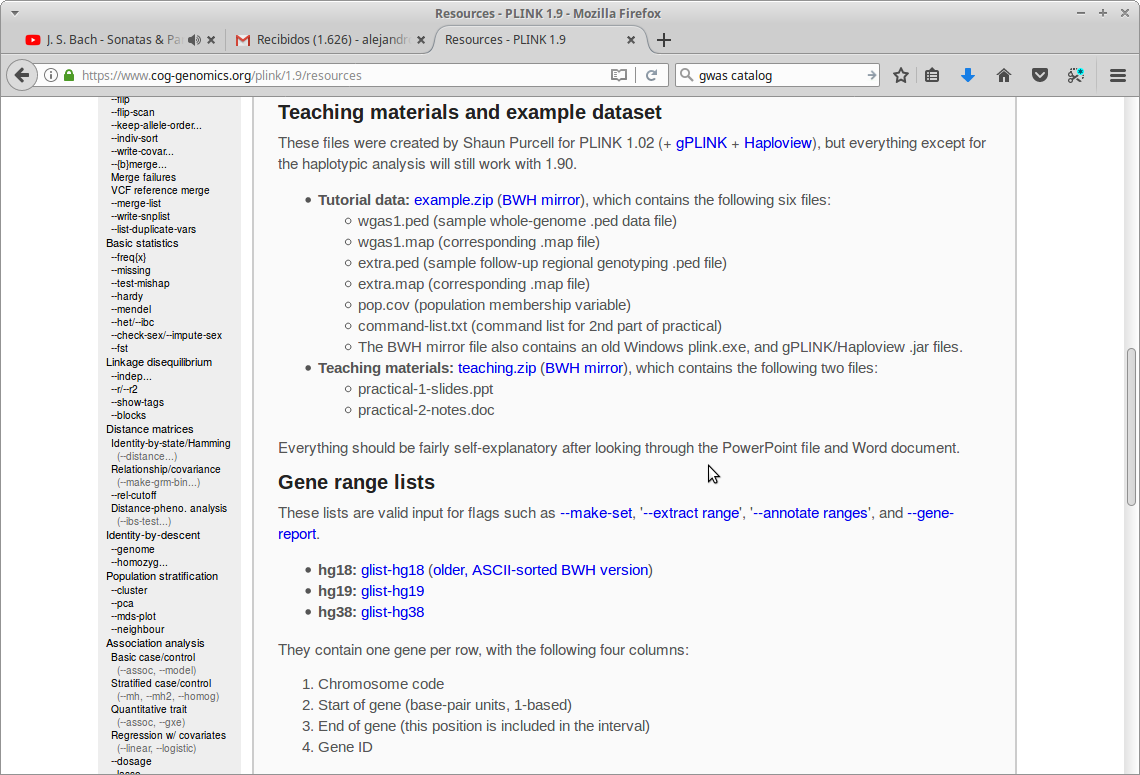
\includegraphics[width=.8\linewidth]{plink.png}
\end{center}
\end{figure}


\end{frame}



\begin{frame}[fragile]
\frametitle{snpStats}
Veamos un ejmplo de analis con snpStats \\
Cargamos los genotipos
\begin{knitrout}\footnotesize
\definecolor{shadecolor}{rgb}{0.969, 0.969, 0.969}\color{fgcolor}\begin{kframe}
\begin{alltt}
\hlkwd{library}\hlstd{(}\hlstr{"snpStats"}\hlstd{)}
\end{alltt}


{\ttfamily\noindent\itshape\color{messagecolor}{\#\# Loading required package: survival}}

{\ttfamily\noindent\itshape\color{messagecolor}{\#\# Loading required package: Matrix}}\begin{alltt}
\hlkwd{load}\hlstd{(}\hlstr{"datos/snp.RData"}\hlstd{)}
\hlstd{snp}
\end{alltt}
\begin{verbatim}
## A SnpMatrix with  1500 rows and  439 columns
## Row names:  1 ... 1500 
## Col names:  1 ... 439
\end{verbatim}
\end{kframe}
\end{knitrout}
\end{frame}

\begin{frame}[fragile]
\frametitle{snpStats}
cargamos los fenotipos
\begin{knitrout}\footnotesize
\definecolor{shadecolor}{rgb}{0.969, 0.969, 0.969}\color{fgcolor}\begin{kframe}
\begin{alltt}
\hlstd{phenos}\hlkwb{<-}\hlkwd{read.table}\hlstd{(}\hlstr{"datos/phenosCont.txt"}\hlstd{,}\hlkwc{header}\hlstd{=}\hlnum{TRUE}\hlstd{)}
\hlkwd{head}\hlstd{(phenos)}
\end{alltt}
\begin{verbatim}
##    pop caco           X1          X2           X3
## 1 Pop1    1 -0.045452947  0.02677151  0.028941220
## 2 Pop1    0  0.018036264 -0.03361612 -0.048915896
## 3 Pop1    1  0.001631087  0.03286500  0.004391887
## 4 Pop1    0  0.021977998 -0.05069528 -0.092101747
## 5 Pop1    0 -0.003845641  0.02882352  0.048173898
## 6 Pop1    0  0.017218303 -0.01419022 -0.011262438
\end{verbatim}
\end{kframe}
\end{knitrout}
\end{frame}

\begin{frame}[fragile]
\frametitle{snpStats}
An\'alisis de asociaci\'on
\begin{knitrout}\footnotesize
\definecolor{shadecolor}{rgb}{0.969, 0.969, 0.969}\color{fgcolor}\begin{kframe}
\begin{alltt}
\hlstd{results} \hlkwb{<-} \hlkwd{snp.rhs.tests}\hlstd{(phenos}\hlopt{$}\hlstd{caco}\hlopt{~}\hlnum{1}\hlstd{,} \hlkwc{snp.data}\hlstd{=snp)}
\hlstd{results[}\hlnum{1}\hlopt{:}\hlnum{10}\hlstd{]}
\end{alltt}
\begin{verbatim}
##    Chi.squared Df     p.value
## 1   10.4005458  1 0.001259781
## 2    8.3516844  1 0.003853300
## 3    2.5211014  1 0.112332103
## 4   12.1936022  1 0.000479537
## 5    0.8892616  1 0.345677499
## 6    2.2825407  1 0.130837388
## 7    0.2688703  1 0.604090611
## 8    0.4893109  1 0.484234857
## 9    4.7639765  1 0.029061334
## 10   3.2426563  1 0.071744229
\end{verbatim}
\end{kframe}
\end{knitrout}
en la sintaxis se omite efecto de interes de los SNPs en la correlaci\'on.

\end{frame}


\begin{frame}[fragile]
\frametitle{snpStats}

El Q-Q plot compara los p-valores obtenidos con los p-vlaores que esperar\'iamos por azar
\begin{knitrout}\footnotesize
\definecolor{shadecolor}{rgb}{0.969, 0.969, 0.969}\color{fgcolor}\begin{kframe}
\begin{alltt}
\hlkwd{qq.chisq}\hlstd{(}\hlkwd{chi.squared}\hlstd{(results),} \hlnum{1}\hlstd{)}
\end{alltt}
\begin{verbatim}
##          N    omitted     lambda 
## 439.000000   0.000000   2.124386
\end{verbatim}
\end{kframe}
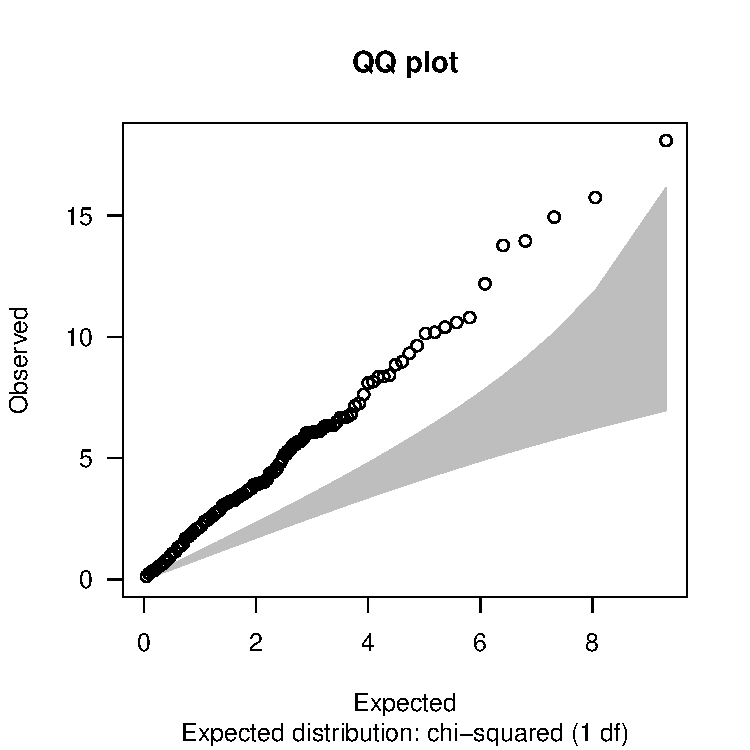
\includegraphics[width=.45\linewidth]{figure/plot1-1} 

\end{knitrout}
vamos que los p-vlaores obtenidos son t\'ipicamente mas altos, est\'an inflados.
\end{frame}

\begin{frame}[fragile]
\frametitle{Correcci\'on por estratificaci\'on poblacional}
Si el fenotipo se correlaciona con la ancestr\'ia y esta es detectada por los SNPs, los valores de correlaci\'on entre fenotipo y SNPs est\'an confundidos porla ancestr\'ia. Debemos corregir por la ancestr\'a como una covariable.   

\end{frame}


\begin{frame}[fragile]
\frametitle{Correcci\'on por estratificaci\'on poblacional}
Incluimos la ancestria pop en la asociaci\'on
\begin{knitrout}\footnotesize
\definecolor{shadecolor}{rgb}{0.969, 0.969, 0.969}\color{fgcolor}\begin{kframe}
\begin{alltt}
\hlstd{resultsAd} \hlkwb{<-} \hlkwd{snp.rhs.tests}\hlstd{(phenos}\hlopt{$}\hlstd{caco}\hlopt{~}\hlstd{phenos}\hlopt{$}\hlstd{pop,} \hlkwc{snp.data}\hlstd{=snp)}
\hlkwd{qq.chisq}\hlstd{(}\hlkwd{chi.squared}\hlstd{(resultsAd),} \hlnum{1}\hlstd{)}
\end{alltt}
\begin{verbatim}
##          N    omitted     lambda 
## 439.000000   0.000000   1.008353
\end{verbatim}
\end{kframe}
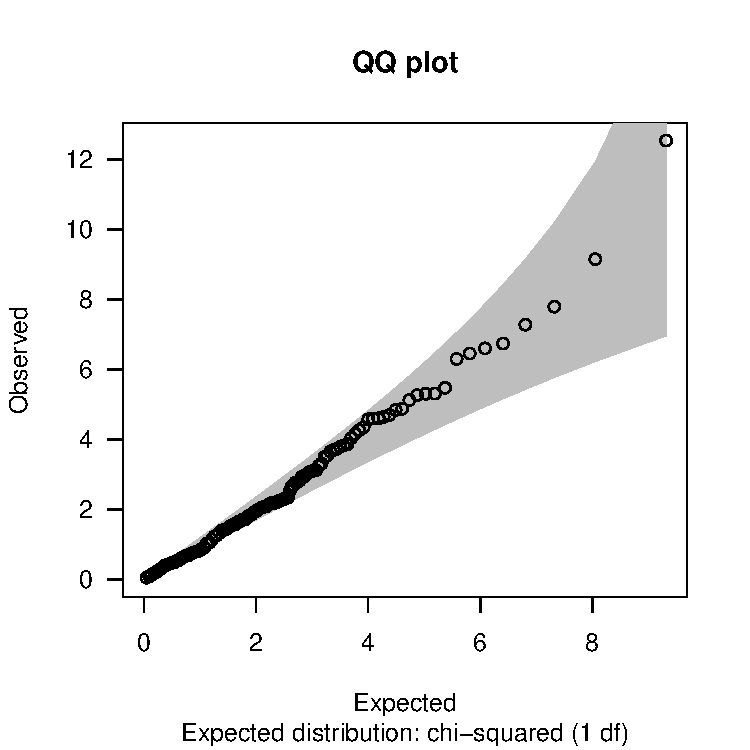
\includegraphics[width=.45\linewidth]{figure/plot2-1} 

\end{knitrout}

\end{frame}


\begin{frame}[fragile]
\frametitle{Correcci\'on por estratificaci\'on poblacional}
Si no tenemos los datos de ancestr\i'a los podemos inferir de la PCA de los SNPs
\begin{knitrout}\footnotesize
\definecolor{shadecolor}{rgb}{0.969, 0.969, 0.969}\color{fgcolor}\begin{kframe}
\begin{alltt}
\hlstd{snpnum}\hlkwb{<-}\hlkwd{matrix}\hlstd{(}\hlkwd{as.numeric}\hlstd{(snp),}\hlkwc{ncol}\hlstd{=}\hlkwd{ncol}\hlstd{(snp))}
\hlstd{d}\hlkwb{<-}\hlkwd{dist}\hlstd{(snpnum,} \hlkwc{method}\hlstd{=}\hlstr{"manhattan"}\hlstd{)}
\hlstd{mds}\hlkwb{<-} \hlkwd{cmdscale}\hlstd{(d,}\hlkwc{eig}\hlstd{=}\hlnum{TRUE}\hlstd{,} \hlkwc{k}\hlstd{=}\hlnum{2}\hlstd{)}\hlopt{$}\hlstd{points}
\hlkwd{plot}\hlstd{(mds,}\hlkwc{col}\hlstd{=phenos}\hlopt{$}\hlstd{pop)}
\end{alltt}
\end{kframe}
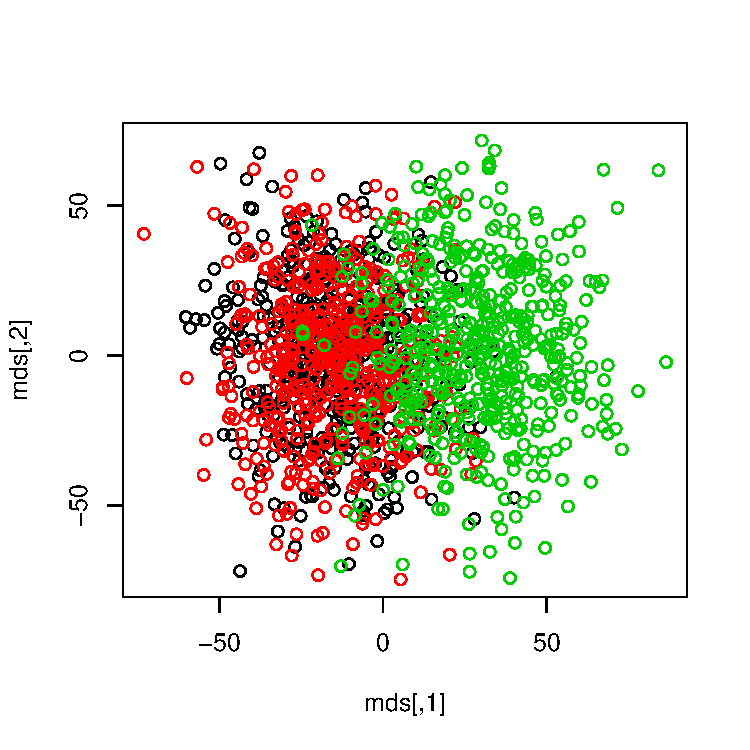
\includegraphics[width=.45\linewidth]{figure/plot3-1} 

\end{knitrout}
\end{frame}

\begin{frame}[fragile]
\frametitle{Correcci\'on por estratificaci\'on poblacional}
Incluimos PCAs en la asociaci\'on
\begin{knitrout}\footnotesize
\definecolor{shadecolor}{rgb}{0.969, 0.969, 0.969}\color{fgcolor}\begin{kframe}
\begin{alltt}
\hlstd{resultsAdPCA} \hlkwb{<-} \hlkwd{snp.rhs.tests}\hlstd{(phenos}\hlopt{$}\hlstd{caco}\hlopt{~}\hlstd{mds[,}\hlnum{1}\hlstd{]}\hlopt{+}\hlstd{mds[,}\hlnum{2}\hlstd{],} \hlkwc{snp.data}\hlstd{=snp)}

\hlkwd{qq.chisq}\hlstd{(}\hlkwd{chi.squared}\hlstd{(resultsAdPCA),} \hlnum{1}\hlstd{)}
\end{alltt}
\begin{verbatim}
##          N    omitted     lambda 
## 439.000000   0.000000   1.403764
\end{verbatim}
\end{kframe}
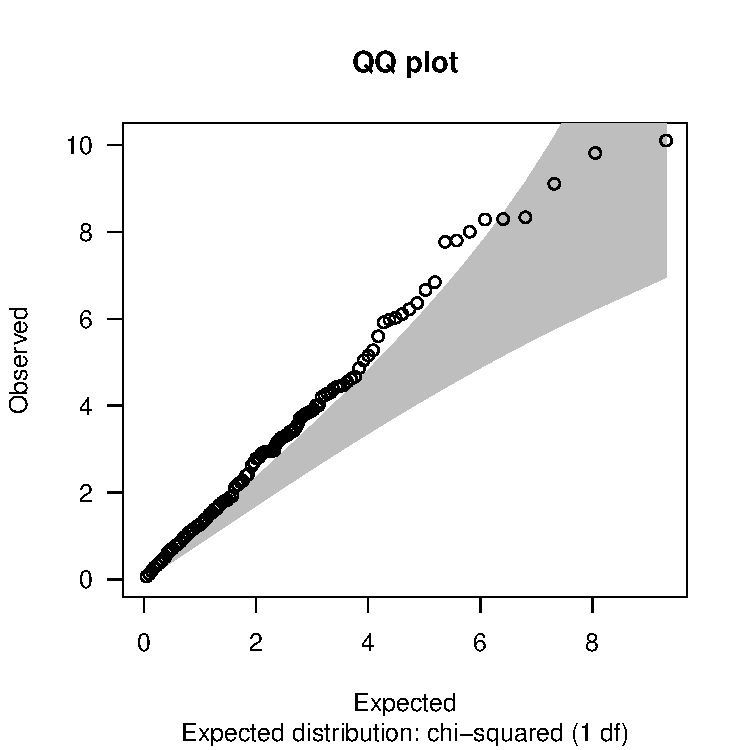
\includegraphics[width=.45\linewidth]{figure/plot4-1} 

\end{knitrout}
\end{frame}

\begin{frame}[fragile]
\frametitle{associaci\'on en R}
Para tener mas control en las asociaciones se pueden usar las funciones b\'asicas de R como {\tt glm}.
\begin{knitrout}\footnotesize
\definecolor{shadecolor}{rgb}{0.969, 0.969, 0.969}\color{fgcolor}\begin{kframe}
\begin{alltt}
\hlstd{mod}\hlkwb{<-}\hlkwd{glm}\hlstd{(phenos}\hlopt{$}\hlstd{caco}\hlopt{~}\hlstd{snpnum[,}\hlnum{1}\hlstd{]}\hlopt{+}\hlstd{mds[,}\hlnum{1}\hlstd{]}\hlopt{+}\hlstd{mds[,}\hlnum{2}\hlstd{],} \hlkwc{family}\hlstd{=}\hlstr{"binomial"}\hlstd{)}
\hlkwd{summary}\hlstd{(mod)}
\end{alltt}
\begin{verbatim}
## 
## Call:
## glm(formula = phenos$caco ~ snpnum[, 1] + mds[, 1] + mds[, 2], 
##     family = "binomial")
## 
## Deviance Residuals: 
##     Min       1Q   Median       3Q      Max  
## -2.3609  -1.0972   0.5874   0.9943   1.8875  
## 
## Coefficients:
##              Estimate Std. Error z value Pr(>|z|)    
## (Intercept)  0.626509   0.161892   3.870 0.000109 ***
## snpnum[, 1] -0.160589   0.077518  -2.072 0.038300 *  
## mds[, 1]     0.029849   0.002320  12.864  < 2e-16 ***
## mds[, 2]     0.002336   0.002175   1.074 0.282769    
## ---
## Signif. codes:  0 '***' 0.001 '**' 0.01 '*' 0.05 '.' 0.1 ' ' 1
## 
## (Dispersion parameter for binomial family taken to be 1)
## 
##     Null deviance: 2054.8  on 1499  degrees of freedom
## Residual deviance: 1844.5  on 1496  degrees of freedom
## AIC: 1852.5
## 
## Number of Fisher Scoring iterations: 4
\end{verbatim}
\end{kframe}
\end{knitrout}
\end{frame}

\begin{frame}[fragile]
\frametitle{associaci\'on en R}
la informaci\'on para la asociaci\'on del primer SNP se exptrae como
\begin{knitrout}\footnotesize
\definecolor{shadecolor}{rgb}{0.969, 0.969, 0.969}\color{fgcolor}\begin{kframe}
\begin{alltt}
\hlstd{summod}\hlkwb{<-}\hlkwd{summary}\hlstd{(mod)}
\hlstd{summod}\hlopt{$}\hlstd{coeff}
\end{alltt}
\begin{verbatim}
##                 Estimate  Std. Error   z value     Pr(>|z|)
## (Intercept)  0.626509309 0.161892007  3.869921 1.088705e-04
## snpnum[, 1] -0.160589175 0.077518112 -2.071634 3.829956e-02
## mds[, 1]     0.029849020 0.002320284 12.864380 7.141304e-38
## mds[, 2]     0.002336155 0.002174946  1.074121 2.827686e-01
\end{verbatim}
\begin{alltt}
\hlstd{summod}\hlopt{$}\hlstd{coeff[}\hlnum{2}\hlstd{,}\hlkwd{c}\hlstd{(}\hlnum{1}\hlstd{,}\hlnum{4}\hlstd{)]}
\end{alltt}
\begin{verbatim}
##    Estimate    Pr(>|z|) 
## -0.16058917  0.03829956
\end{verbatim}
\end{kframe}
\end{knitrout}
\end{frame}

\begin{frame}[fragile]
\frametitle{associaci\'on en R}
La informaci\'on para todos los SNPs.
\begin{knitrout}\footnotesize
\definecolor{shadecolor}{rgb}{0.969, 0.969, 0.969}\color{fgcolor}\begin{kframe}
\begin{alltt}
\hlstd{pvals}\hlkwb{<-}\hlkwd{sapply}\hlstd{(}\hlnum{1}\hlopt{:}\hlkwd{ncol}\hlstd{(snpnum),} \hlkwa{function}\hlstd{(}\hlkwc{j}\hlstd{)}
\hlstd{\{}
  \hlstd{mod}\hlkwb{<-}\hlkwd{glm}\hlstd{(phenos}\hlopt{$}\hlstd{caco}\hlopt{~}\hlstd{snpnum[,j]}\hlopt{+}\hlstd{mds[,}\hlnum{1}\hlstd{]}\hlopt{+}\hlstd{mds[,}\hlnum{2}\hlstd{],} \hlkwc{family}\hlstd{=}\hlstr{"binomial"}\hlstd{)}
  \hlstd{summod}\hlkwb{<-}\hlkwd{summary}\hlstd{(mod)}
  \hlstd{summod}\hlopt{$}\hlstd{coeff}
  \hlstd{summod}\hlopt{$}\hlstd{coeff[}\hlnum{2}\hlstd{,}\hlkwd{c}\hlstd{(}\hlnum{1}\hlstd{,}\hlnum{4}\hlstd{)]}
\hlstd{\})}
\hlkwd{head}\hlstd{(}\hlkwd{t}\hlstd{(pvals))}
\end{alltt}
\begin{verbatim}
##         Estimate    Pr(>|z|)
## [1,] -0.16058917 0.038299564
## [2,] -0.11357896 0.139997189
## [3,] -0.09533903 0.203844762
## [4,] -0.21930524 0.004046846
## [5,]  0.03336892 0.669076533
## [6,]  0.09750542 0.225846032
\end{verbatim}
\end{kframe}
\end{knitrout}
\end{frame}


\begin{frame}[fragile]
\frametitle{associaci\'on en R}
Los resultados son id\'enticos a los obtenidos con snpStats

\begin{knitrout}\footnotesize
\definecolor{shadecolor}{rgb}{0.969, 0.969, 0.969}\color{fgcolor}\begin{kframe}
\begin{alltt}
\hlkwd{plot}\hlstd{(}\hlkwd{p.value}\hlstd{(resultsAdPCA), pvals[}\hlnum{2}\hlstd{,])}
\end{alltt}
\end{kframe}
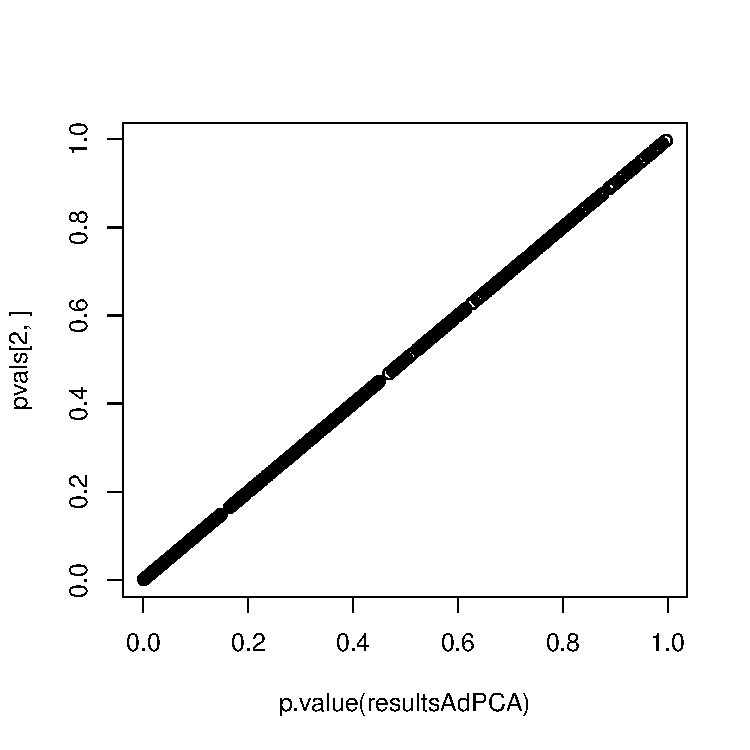
\includegraphics[width=.45\linewidth]{figure/plot5-1} 

\end{knitrout}
\end{frame}


\begin{frame}[fragile]
\frametitle{Genome-wide association studies}
Elementos importantes a considerar.

\begin{itemize}
\item Usamos p-valores para identificar los SNPs que mas se correlacionan con el fenotipo
\item la verdadera hip\'otesis del estudio es si existe \emph{alg\'un} SNP que se correlacione con el fenotipo
\item si nos creemos SNPs con $p<0.05$ entonces siempre identificar\'iamos al rededor de $5\%$ de asociaciones significativas, que son realmente puro azar. 
\item tememos que ajustar por el n\'umero de SNPs que probamos y creernos solo $p=0.05/nunSNPs$
\item en GWAS de 1 millon de SNPs esto significa  $p<10^{-8} $
\end{itemize}

\end{frame}



\begin{frame}[fragile]
\frametitle{Ejercicio}

\begin{itemize}
\item Estudio de asociaci\'on en c\'odigo R si ajustamos por la ancestr\'ia dada por la variable {\tt pop} en {\tt phenos}.
\item comparar con los pvalores que obtuvimos antes
\item Qu\'e podemos decir en t\'erminos de poder estad\'istico y falsos positivos?
\end{itemize}

\end{frame}


\begin{frame}[fragile]
\frametitle{Ejercicio}

\begin{knitrout}\footnotesize
\definecolor{shadecolor}{rgb}{0.969, 0.969, 0.969}\color{fgcolor}\begin{kframe}
\begin{alltt}
\hlstd{pvalsPop}\hlkwb{<-}\hlkwd{sapply}\hlstd{(}\hlnum{1}\hlopt{:}\hlkwd{ncol}\hlstd{(snpnum),} \hlkwa{function}\hlstd{(}\hlkwc{j}\hlstd{)}
\hlstd{\{}
  \hlstd{mod}\hlkwb{<-}\hlkwd{glm}\hlstd{(phenos}\hlopt{$}\hlstd{caco}\hlopt{~}\hlstd{snpnum[,j]}\hlopt{+}\hlstd{phenos}\hlopt{$}\hlstd{pop,} \hlkwc{family}\hlstd{=}\hlstr{"binomial"}\hlstd{)}
  \hlstd{summod}\hlkwb{<-}\hlkwd{summary}\hlstd{(mod)}
  \hlstd{summod}\hlopt{$}\hlstd{coeff}
  \hlstd{summod}\hlopt{$}\hlstd{coeff[}\hlnum{2}\hlstd{,}\hlkwd{c}\hlstd{(}\hlnum{1}\hlstd{,}\hlnum{4}\hlstd{)]}
\hlstd{\})}
\end{alltt}
\end{kframe}
\end{knitrout}
\end{frame}

\begin{frame}[fragile]
\frametitle{Ejercicio}

\begin{knitrout}\footnotesize
\definecolor{shadecolor}{rgb}{0.969, 0.969, 0.969}\color{fgcolor}\begin{kframe}
\begin{alltt}
\hlkwd{plot}\hlstd{(pvals[}\hlnum{2}\hlstd{,],pvalsPop[}\hlnum{2}\hlstd{,])}
\end{alltt}
\end{kframe}
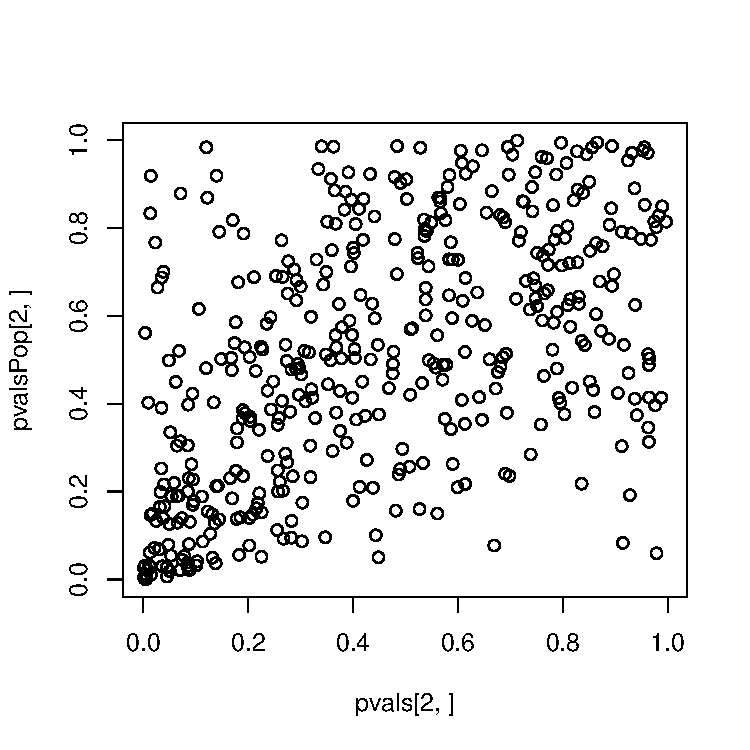
\includegraphics[width=.45\linewidth]{figure/plot6-1} 

\end{knitrout}
\end{frame}


\end{document}
